\documentclass[a4paper,10pt]{article}
\usepackage[utf8]{inputenc}
\usepackage{listings}
\usepackage[portuguese]{babel}
\usepackage{graphicx}
\usepackage{natbib}
\usepackage{subfig}
\title{Uma abordagem MPI para transcrição e tradução de cadeias de DNA}
\author{Daniel Arena, Erick Grilo, Eduardo Loivos, Max Fratane}
%http://www.math.tu-cottbus.de/~kd/parallel/mpi/mpi-course.book_38.html
\lstset{extendedchars=\true}
\lstset{inputencoding=ansinew}

\begin{document}
\begin{flushright}
\thispagestyle{empty}
\includegraphics[width=.2\textwidth]{IC-UFF.pdf}
\end{flushright}

\begin{center}
\vfill
\vspace{-7em}
\emph{\Large Uma abordagem MPI para transcrição e tradução de DNA}
\begin{flushright}
\vspace{1em}
\makebox[.5\textwidth][l]{\parbox{.5\textwidth}{
\vspace{2em}
Elihofni Lima\\
Erick Grilo\\ 
Max Fratane\\ 
}}
\end{flushright}
\vfill
\end{center}

\newpage
\newpage

\section{Introdução e descrição da aplicação}
\paragraph{}A transcrição do DNA é o processo através do qual o DNA serve de modelo para a síntese de RNA feita por um ser vivo. Apenas uma cadeia de DNA é usada nesse processo, ativada pela enzima RNA-polimerase. Em uma determinada região da molécula de DNA, ocorre a separação das hélices, onde uma delas forma o RNA através do encadeamento de nucleotídeos complementares. Em suma, essa é a fase responsável por parear as bases nitrogenadas do DNA com as do RNA: A do DNA com U do RNA, T do DNA com A do RNA, C do DNA com G do Rna e G do DNA com C do RNA.

\paragraph{}Relembrando alguns conceitos de biologia, A (adenina), C (citosina) T (timina) e G (guanina) são os nucleotídeos que compõem o DNA, e as mesmas, com exceção da timina (que vira U, de uracila, que por sua vez é uma base nitrogenada), compõem o RNA. Cada trinca de 3 dessas bases nitrogenadas é chamada de códons. Um códon codifica um aminoácido, vide \citet{objetivo}.

\paragraph{}Motivado pelo tamanho que uma cadeia de DNA pode ter (em \citet{venter2001sequence}, no mapeamento do genoma humano, por exemplo, foram encontradas aproximadamente 2.91 bilhões de pares de bases nitrogenadas) e pelo processo de transcrição ser uma tarefa repetitiva, a criação de um programa paralelo do tipo SPMD (Simple Program, Multiple Data) aparenta ser uma boa abordagem para a solução desta tarefa. \citet{chibli2008multiprocessor} nos dá uma abordagem usando MPI para solucionar problemas de comparação de \emph{strings}, incluindo a transcrição de DNA para RNA e a identificação de aminoáciods, enquanto em \citet{kleinjung2002parallelized} e \citet{xue2014parallel}, o padrão MPI é utilizado para outro fim, que é o alinhamento de sequências de DNA (que visa encontrar similaridades no DNA que podem indicar relações evolucionárias entre diferentes indivíduos, ou seja, características semelhantes entre indivíduos de espécies diferentes.)\\ 
\paragraph{}O objetivo é paralelizar a transcrição e a tradução de DNA, onde a transcrição é o processo responsável por traduzir uma cadeia de DNA para RNA e a tradução consiste em identificar o aminoácido que o códon em questão representa, a partir de códons de RNA (que foram obtidos a partir da trascrição de códons de DNA para RNA). Note que o processo só se inicia efetivamente quando na cadeia original de DNA dado na entrada é identificado um cístron (uma cadeia de DNA iniciada pelos códons compostos por ATC, ACT ou ATT, que possui informações para a síntese de uma proteína). Enquanto um cístron não é encontrado, não há nenhum processamento efetivo. Quando um cístron é encontrado, o processo se inicia. Como estamos considerando nenhuma mutação genética, o tamanho do cístron deve ser um número múltiplo de 3 para que o algoritmo funcione corretamente. A cadeia original pode ter qualquer tamanho.\\
\newpage

\section{A implementação sequencial}

\paragraph{}O método sequencial consiste em tratar toda a cadeia de entrada como uma única cadeia, oriunda da leitura de um arquivo texto onde se encontra tal cadeia. A partir daí, toda a cadeia do DNA é transcrita para RNA da seguinte forma: primeiramente, é identificada o local correto para iniciar a transcrição da cadeia (onde o cístron se encontra). A cadeia então é subdividida em grupos de três bases nitrogenadas (um códon) e em seguida, a cada códon, sua transcrição (conversão de DNA para RNA) é feita e a identificação do aminoácido que aquele códon se refere é feita em seguida. Ao término da análise de um códon, o códon DNA original, a sua transcrição para códon RNA e o aminoácido que ele representa é escrito em uma linha do arquivo e esse procedimento se repete por todo o tamanho da cadeia de entrada. Caso o códon não possui 3 nucleotídeos (o tamanho do cístron não é múltiplo de 3), tal codon é ignorado. \\

Para a execução da aplicação sequencial, usa-se:
\begin{center}\begin{itemize}\item{Compilar:} `gcc main-seq.c transcription.c io.c -o dna-seq`\\
    \item{Executar:} `./dna-seq` \end{itemize}\end{center}

\begin{figure}[!htb]
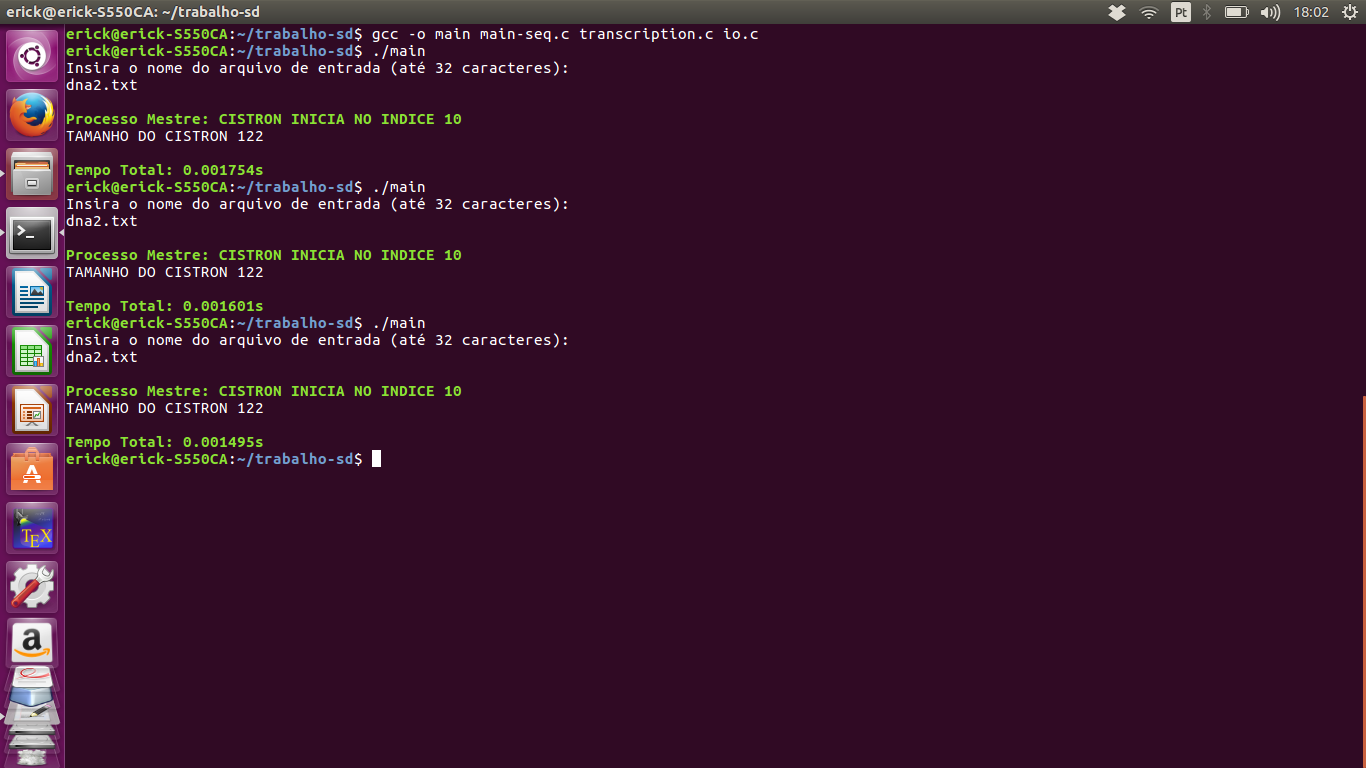
\includegraphics[scale=0.30]{execucao1.png}
\caption{Exemplo de uma execução da aplicação sequencial, indicando onde o cístron é encontrado na cadeia origina, seu tamanho e o tempo total de execução.}
\label{seq}
\end{figure}
\newpage


\section{A implementação paralela}

\paragraph{}O método paralelo consiste em paralelizar todo o processo de transcrição de DNA em RNA e o de tradução do códon para um aminoácido. Dessa forma, o trabalho é divido em n tarefas (1 tarefa mestre, n-1 tarefas escravo) onde a tarefa mestre é a responsável por repartir a sequência de DNA de entrada para as demais tarefas, ficando com a primeira parte da sequência. Após o envio dessas partes da entrada para cada uma das tarefas escravo, a tarefa mestre faz a transcrição da sua parcela da sequência de DNA para RNA, ao mesmo tempo que as tarefas escravo (após receberem a mensagem que contém os dados da tarefa mestre) também iniciam esse processo. A tarefa mestre então realiza a identificação dos aminoácidos que ela transcreveu e fica aguardando as demais tarefas escravo realizarem a parcela do seu processamento (transcrever e identificar os aminoácidos que lhe foram enviadas).\\
\paragraph{}Quando todas as tarefas escravo terminarem o seu processamento, elas enviam de volta os resultados para a tarefa mestre (os códons transcritos e os aminoácidos identificados), que por sua vez imprime na tela o RNA transcrito e os aminoácidos identificados e escreve em um arquivo tais dados.

\begin{figure}[!htb]
\centering
\subfloat[Início da execução, mostrando o \emph{status} dos processos, tamanho total da cadeia de entrada, tamanho do cístron que será processado, o total de códons, a quantidade de códons enviados para cada processo escravo e parte do resultado final.]{
\includegraphics[scale=0.28]{par1.png}
\label{par1}
}
\quad
\subfloat[Fim da execução, mostrando a confirmação do recebimento dos dados processados pela tarefa mestre, os dados processados (que foram escritos em um arquivo e o tempo total de execução]{
\includegraphics[scale=0.28]{par2.png}
\label{par2}
}
\caption{Exemplo de uma execução da aplicação paralela, no ambiente MPI com dois processos, um mestre e um escravo}
\label{Figura 1}
\end{figure}

\newpage

\section{A implementação paralela}
\subsection{Ferramentas}

\paragraph{}O ambiente escolhido para a paralelização da implementação foi o MPI (\emph{Message Passing Interface}, um padrão de comunicação de dados em computação paralela cujo objetivo busca efetuar a troca de mensagens entre processos ou threads, dependendo da implementação) de fomra prática e eficiente. A implementação do padrão MPI utilizada é a OpenMPI \citep{gabriel2004open} escrito em C e a linguagem utilizada é C .\\
\paragraph{} A nossa implementação consiste no uso do ambiente MPI para paralelizar o processo: Ao iniciar o ambiente MPI, o ambiente de execução paralela é inicalizado. Em seguida, as tarefas são criadas e inicializadas no comunicador padrão (MPI\_COMM\_WORLD) e, então, existem duas rotinas possíveis para serm executadas por cada uma das tarefas, que é a rotina destinada para a tarefa mestre (identificada pelo rank 0) e outra para as demais tarefas (cujo identificadores variam de 1 a N-1, N sendo o número de processos).\\

No padrão MPI na implementação OpenMPI, as principais características são:
\begin{itemize}
\item{Transparência}: O padrão MPI fornece transparência de acesso (Fica transparente ao usuário como as máquinas acessam um dado recurso), transparência de concorrência: no MPI, chamadas síncronas podem ser feitas usando os comandos \emph{MPI\_Send} (envio de mensagens) e \emph{MPI\_Recv} (recebimento de mensagens) cuja implementação é transparente ao usuário. Vale notar que o MPI também fornece chamads assíncronas porém o padrão MPI não fornece transparência de localização, de migração  nem de relocação  (para fazer uso de várias máquinas com uma aplicação MPI, é necessário ter um arquivo com os endereços IP das máquinas onde os processos MPI irão executar. Ou seja, é necessário saber a localização física das máquinas e as máquinas não podem se movimentar) e nem transpareência de falha: a tolerância a falhas em MPI é zero (em uma aplicação MPI, se um processo falha, todo o \emph{job} (a aplicação) MPI falha (é abortada).

\item{Comunicação}: O padrão MPI utiliza a ideia de comunicação orientada à mensagens. O padrão MPI foi criado para resolver problemas que a comunicação via \emph{sockets} não tratavam muito bem, como o seu uso em protocolos proprietários de alta velocidade.\\
No padrão MPI, a comunicação se dá em um grupo de processos conhecidos chamado de comunicador (tal grupo é designado pela diretiva MPI\_COMM\_WORLD, que é o chamado comunicador universal (padrão) dos processos de uma aplicação MPI. Tal comunicador contém todos os processos MPI e é criado na inicialização do ambiente MPI por meio da diretiva MPI\_INIT. Usando o MPI\_COMM\_WORLD, todos os processos envolvidos na aplicação MPI conhecem todos os processos, podendo qualquer processo se comunicar com um outro processo dentro do mesmo comunicador. Vale notar que no geral, é possível uma aplicação MPI possuir mais de um comunicador, onde um processo pode pertencer à mais de um comunicador, podendo ter diferentes \emph{ranks} em diferentes comunicadores.\\

A troca de mensagens entre diferentes processos usa o identificador do grupo do processo e o rank do processo para identificar fonte ou destinatário de uma dada mensagem. Por exemplo, na chamada:\\
\begin{center} MPI\_Recv (buf, count, datatype, src, tag, comm,status)\\ \end{center}
que é uma rotina de recebimento bloqueante do \emph{MPI}, \emph{buf} é a variável que contém o dado,  \emph{count} é a quantidade de dados que está sendo enviada na mensagem, \emph{datatype} é o tipo de dado que está sendo enviado, \emph{src} é o rank do processo que está enviando (a fonte) a mensagem, \emph{tag} é o índice da mensagem, \emph{comm} é o comunicador ao qual o processo pertence e \emph{status} é uma variável do tipo MPI\_Status que vai armazenar o status do sistema após tal operação.\\

Existem quatro modelos de comunicação fornecidos pelo MPI: padrão, síncrona, \emph{bufferizada} e assíncrona. Tais modos diferem no modo que a mensagem é enviada. O envio padrão é dado pelo uso da rotina MPI\_Send, que envia de uma forma bloqueante, bloqueando o processo até que a mensagem seja enviada para o destino. O envio síncrono é dado pela rotina MPI\_SSend, que possui apenas uma diferença frente ao MPI\_Send: enquanto MPI\_send não aguarda o receptor receber a mensagem para desbloquear, MPI\_SSend aguarda a mensagem chegar no destinatário para desbloquear sua rotina. Já o envio bufferizado copia a mensagem para um buffer de sistema para transmissão posterior se necessário. Ao usar esse tipo de chamada, o programador deve especificar o tamanho do buffer à priori usando a diretiva MPI\_BUFFER\_ATTACH(buffer,size), onde \emph{buffer} é o bufer e \emph{size} é o tamanho do buffer e o envio assíncrono consiste em enviar a mensagem imediatamente, jogando-a no comunicador e (literalmente) torcer para que o processo receptor receba a mensagem, onde tal processo pode ou não receber a mensagem.

É utilizado o envio padrão (bloqueante) na nossa aplicação por ser o mais simples e necessário para a aplicação.\\


\item{Nomeação}: A nível lógico, o padrão MPI usa o conceito de \emph{ranks} para identificar seus processos. Na implementação OpenMPI, os processos possuem \emph{ranks} que são enumerados de zero à N-1 (N sendo o número total de processos da aplicação MPI)  e os \emph{ranks} são os identificadores de um processo dentro de um dado comunicador. Por padrão, costuma-se usar (em abordagens do tipo coordenador-trabalhador) o rank 0 como sendo o coordenador e os demais ranks são os processos operários.\\

\item{Sincronização} O MPI possui uma rotina específica chamda MPI\_Barrier(MPI\_Comm communicator) que sincroniza todos os processos que fazem parte do comunicador \emph{communicator}, criando uma espécie de barreira onde a execução dos processos só continua quando todos eles atingirem o mesmo ponto. Tal sincronização é transparente ao programador que usa o padrão MPI.

\item{Tolerância a falhas} MPI não tolera falhas: quedas de processos e/ou de mensagens trocadas entre processos ocasionam a interrupção do funcionamento da aplicação MPI como um todo.


\end{itemize}
\subsection{Descrição da implementação}
\paragraph{}A tarefa mestre então inicia sua execução: primeiro ela efetua a leitura do arquivo (utilizando a função \emph{ler}, disponível em io.c), obtendo a cadeia de DNA inserida como entrada e, em seguida, dividindo a mesma em pedaços menores de sub-cadeias de DNA (por exemplo, para uma cadeia de 60 nucleotídeos, como cada códon possui tamanho 3, nessa etapa a tarefa mestre dividiria a cadeia em 20 sub-cadeias de tamanho 3 cada, utilizando a rotina split, encontrada em transcription.c) e em seguida, envia as subcadeias para as demais tarefas (mantendo a primeira porção para si) por meio da chamada da função MPI\_Send (primeiramente enviando a quantidade de códons que a tarefa irá receber, em seguida enviando os códons), que faz o envio bloqueante síncrono de mensagens (isso significa que a tarefa que está enviando retorna a execução assim que a mensagem foi enviada, o que não implica que a mesma foi recebida pela tarefa receptora).\\
\paragraph{}Após o envio dos dados necessários (quantidade de códons e os códons em si), a tarefa mestre começa a efetuar o processamento na parte dos códons que com ela ficou: primeiro, ela divide a sub-cadeia de DNA que restou em outras sub-cadeias de tamanho 3 (o tamanho de um códon) e, para cada uma dessas sub-cadeias, faz a transcrição de DNA para RNA, utilizando a função transcription (encontrada em transcription.c) e em seguida identificando o aminoácido referente ao códon transcrito, fazendo uso da rotina transcription (que pode ser encontrada em trascription.c).\\
\paragraph{}Nesse momento, as demais tarefas escravo também estão fazendo o mesmo: após o recebimento das mensagens que foram enviadas pela tarefa mestre (recebimento feito por meio da rotina MPI\_Recv), cada uma das tarefas escravo divide a cadeia de DNA recebida em sub-cadeis de tamanho 3 (da mesma forma que a mestre), e, para cada sub-cadeia de DNA gerada a partir da cadeia que a tarefa recebeu, ela faz a transcrição de DNA e a tradução do códon para o aminoácido que ele identifica (da mesma forma que a tarefa mestre). Ao término do processo, elas enviam o resultado do processamento (que seria todos os códons transcritos e cada um dos seus respectivos aminoácidos) para a tarefa mestre\\
\paragraph{} A mestre então, para cada tarefa escravo, ela recebe os dados da tarefa escravo (por meio da rotina MPI\_Recv) e, para cada conjunto de dados recebidos (de cada tarefa), ela vai armazenando as cadeias de RNA transcritos e os seus respectivos aminoácidos. Ao fim da recepção (todas as tarefas escravo concluíram o envio, a tarefa mestre então imprime na tela o resultado do processamento: para cada códon, imprime na tela o códon de DNA original da entrada, a cadeia de RNA transcrita referente à tal códon e o aminoácido que tal cadeia de RNA identifica. Em seguida, escreve o mesmo que ela imprimiu em um arquivo de saída. Ao fim da execução do ambiente MPI, é pego o tempo de finalização (a fim de ver quanto tempo o processamento levou) e o ambiente é finalizado pelo processo main (o mesmo onde o ambiente é inicializado) por meio da rotina MPI\_Finalize.\\

Para executar a aplicação paralela (em uma única máquina), usa-se:
\begin{center}\begin{itemize}\item{Compilar:} `mpicc main-mpi.c transcription.c io.c -o dna-mpi`\\
                     \item{Executar (x processos):} `mpirun -np x dna-mpi`\end{itemize}\end{center}


\section{Descrição dos experimentos computacionais}
A ideia inicial seria efetuar a medição de desempenho em diversas máquinas. Porém, como não foi possível, a máquina física onde o código foi executado é um computador com 8 GB de memória RAM DDR3, processador Intel i7-5500U (8 núcleos) @ 2.40 GHz, com o S.O Ubuntu 16.04 LTS 64 bit.  Foram executados 2 casos de teste: uma entrada com a cadeia de DNA com 131 bases nitrogenadas, com um cístron de tamanho 122 e uma entrada com  um cístron contendo 2521 bases nitrogenadas
(observe que a quantidade de cístons na entrada pode diferir do tamanho da cadeia de DNA de entrada original).

\begin{table}[!htb]
\begin{tabular}{| l | l | l | l | l | p{5cm} |} 
\hline
  Nº processos & 1ª execução & 2ª execução & 3ª execução & Média\\ \hline
1 processo   &	0.001601s   &   0.001495s   & 0,000170s   &  0.001657s\\ \hline

\end{tabular}
\caption{Tabela da execução com entrada de um cístron com 60 nucleotídeos para a aplicação sequencial}
\end{table}

\begin{table}[!htb]
\begin{tabular}{| l | l | l | l | l | p{5cm} |} 
\hline
  Nº processos & 1ª execução & 2ª execução & 3ª execução & Média\\ \hline
1 processo   &	0.000384s &  0.000669s    & 0.000779s  &  0.000611s \\ \hline
2 processos &	0.000430s & 0.000581s &  0.000417s    &  0.000476s\\ \hline
3 processos & 0.000592s & 0.000389s & 0.000520s &  0.000500  \\ \hline
4 processos & 0.000878s & 0.000730s & 0.000920s  &  0.000842s  \\ \hline
5 processos  &  0.000592s & 0.000389s & 0.000520s  &  0.000600s  \\ \hline
%6 processos & 0,002399s  &  0,006788s  &  0,003720s  &  0,004302s  \\ \hline
%7 processos & 0,009775s  & 0,002534s  &  0,003134s  &  0,005147s\\ \hline
%8 processos & 0,002090s  &  0,005234s  &  0,010324s  &  0,005882s  \\ \hline
%9 processos & 0,006355s  &  0,005824s  &  0,007481s  &  0,006553s \\ \hline
%TODO
10 processos & 0,004734s  &  0,004441s  &  0,015296s  &  0,008157s \\ \hline
%20 processos & 0,007049s  &  0,007616s  &  0,048893s  &  0,021186s \\ \hline 
\end{tabular}
\caption{Tabela da execução com entrada de um cístron com 122 bases nitrogenadas para a aplicação paralela}
\end{table}

Para a prmeira bateria de testes, temos que o resultado da apliação sequencial foi bem satisfatório: em todos os casos onde o número de tarefas é menor do número de núcleos, o desempenho da aplicação usando MPI foi melhor do que a sequencial, pois cada processo roda em um diferente núcleo. Vale notar que quando o número de processos ultrapassa o número de núcleos da máquina, o tempo da aplicação paralela é pior do que todos os demais testes dela e também é pior que o tempo da aplicação sequencial. Uma possível razão é o enfileiramento de mensagens entre os processos (onde para os processos serem executados eles passam a disputar os núcleos da CPU por não ter o suficiente para todos executarem em paralelo simulatenamente, nesse caso.
\newpage
\begin{table}[!htb]
\begin{tabular}{| l | l | l | l | l | p{5cm} |} 
\hline
  Nº processos & 1ª execução & 2ª execução & 3ª execução & Média\\ \hline
1 processo   &	0.021487s  &  0.026066s  &  0.028954s & 0.025502s\\ \hline

\end{tabular}
\caption{Tabela da execução com entrada de um cístron com 2521 bases nitrogenadas para a aplicação sequencial}
\end{table}

\begin{table}[!htb]
\begin{tabular}{| l | l | l | l | l | p{5cm} |} 
\hline
Nº processos & 1ª execução & 2ª execução & 3ª execução & Média\\ \hline
1 processo & 0.006514s & 0.005006s & 0.006639s & 0.005891s \\\hline
2 processos & 0.006936s & 0.005423s &  0.005735s & 0.006031s \\\hline
3 processos & 0.011321s & 0.013001s & 0.011141s & 0.011821s \\\hline
4 processos & 0.010910s & 0.010860s & 0.014518s & 0.012096s \\\hline
6 processos & 0.035180s & 0.034607s & 0.035032s & 0.034940s \\\hline
15 processos & 0.041788s & 0.041012s & 0.038704s & 0.040501s \\\hline
41 procesos & 0.013867s & 0.014117s & 0.021192s & 0.016392s \\\hline
\end{tabular}
\caption{Tabela da execução com entrada de um cístron com 2521 bases nitrogenadas para a aplicação paralela}
\end{table}


Para a segunda bateria de testes, o resultado se mantém: para todos os casos de teste onde a aplicação MPI é executada com menos processos que o número de núcleos de processamento da máquina usada, o desempenho da aplicação paralela usando MPI é melhor do que o desempenho da aplicação sequencial. Surpreendentemente, o resultado da aplicação ao executar com 41 processos (número primo inserido de propósito para fins de teste) foi melhor do que o executado com 6 e com 15 processos, respectivamente. Uma possível explicação pode ser que algum recurso que facilitasse a execução desta aplicação poderia estar sendo usado pelo SO da máquina (ou por uma outra aplicação em execução no plano de fundo) e ao executar a aplicação com 41 processos, já não estava mais.

\section{Conclusões}

Baseados nos dados acima apresentados, somos levados à concluir que o uso do paradigma de programação baseada em troca de mensagens é bem útil para aplicações que necessitam de processamento paralelo para ter um melhor desempenho. O OpenMPI oferece uma implementação robusta do MPI, fornecendo um ambiente de programação usando troca de mensagens de forma eficiente e transparente ao programador que invoca o MPI.



\bibliographystyle{agsm}
\bibliography{bibliografia}
\end{document}
